
\section{Inledning}
Kontrollera alltid alla ytor som ni eller era gäster har nyttjat. Ni som arrangörer är ansvariga för att \textbf{alla} områden som finns med i detta dokument kontrolleras och städas vid behov, även om det inte är ni som har skräpat ner. Vi som arrangerar i Hubben är de enda som ser till att det är städat och det är därför viktigt att vi alla drar vårt strå till stacken så att den inte faller sönder.\\

Detta dokument fungerar främst som riktlinger och behöver inte följas exakt. Om ni tror att det räcker att bara sopa efter ett arrangemang, gör det. Dokumentet ger dock en god insikt i vad vi i P.R.I.T. anser vara ett korrekt städ och det är därför en god idé att checka av alla punkter innan städet anses färdigt.\\

Då städet är färdigt är det bra om ni tar några snabba bilder på alla delar av Hubben för att kunna bevisa att ni faktiskt städade. Det händer att andra personer stökar ner efter att ni har städat.\\

Kontakta P.R.I.T. (prit@chalmers.it) om ni har några frågor eller funderingar.

\section{Allmänt}
Dessa saker görs ofta sist.
\begin{itemize}
    \item Se till att alla moppar är torra (krama ur dem).
    \item Se till att städinventarier är på rätt plats och att de är relativt rena.
    \item Släck alla lampor i Hubben (glöm inte hallen och toaletterna).
    \item Stäng alla fönster i Hubben.
    \item Stäng av och töm kylarna bakom baren. Se till att de lämnas på glänt, annars börjar det lukta illa!
    \item Töm alla ''vanliga'' sopor om de är fulla eller luktar illa. Detta är särskilt viktigt under ledigheter eftersom ni då är de ända som tömmer. Nyckeln till soprummet finns i frum bakom styrIT-skåpet.
    \item Töm glasåtervinning.
    \item Töm metallåtervinning (tyvärr finns inget bra ställe att återvinna metall på, därför får ni antingen gå till återvinningscentralen vid Gibraltargatan eller slänga det i brännbart).
\end{itemize}


\section{Stor-Hubben och hallen}
\begin{itemize}
    \item Tänd de starka lamporna med knappen bredvid baren eller vid toaletterna så att ni ser ordentligt.
    \item Torka av alla bord, stolar och soffor.
    \item Flytta möblerna till studierummet innan ni gör rent golvet.
    \item Rengör golvet.
    \begin{itemize}
        \item Sopa golvet.
        \item Upprepa tills golvet anses rent (vanligtvis en eller två gånger):
        \begin{enumerate}
            \item Moppa golvet med endast varmvatten (använd bara medel om det är fettfläckar som inte går bort efter två vattenmoppningar). Kranen i köket är enklast att fylla på vid samt ger varmast vatten.
            \item Raka golvet.
            \item Töm mopphinkar så fort botten inte syns. Töm i toaletten och spola.
        \end{enumerate}
        \item Moppa med vatten en sista gång och låt det lufttorka (för att undvika märken från rakor).
        \item Töm mopphinkarna i toaletten och spola. Skölj även ur mopphinkarna med vatten en sista gång.
    \end{itemize}
    \item Bär tillbaka alla möblerna och placera dem som de stod innan arret.
    \item Stäng av projektor och se till att bardatorn inte spelar musik.
    \item Torka av och gör rent bardisken.
    \item Dra upp persiennerna.
\end{itemize}

\section{Köket}
\begin{itemize}
    \item Diska all disk, starta diskmaskinen.
    \item Torka av stekplattor (inklusive sladdarna), köksytor och bord med vatten och diskmedel.
    \item Rengör golvet (glöm inte området under kökssoffan).
    \begin{itemize}
        \item Sopa golvet.
        \item Upprepa tills golvet anses rent (vanligtvis en eller två gånger):
        \begin{enumerate}
            \item Moppa golvet med endast varmvatten (använd bara medel om det är fettfläckar som inte går bort efter två vattenmoppningar). Kranen i köket är enklast att fylla på vid samt ger varmast vatten.
            \item Raka golvet.
            \item Töm mopphinkar så fort botten inte syns. Töm i toaletten och spola.
        \end{enumerate}
        \item Töm mopphinkarna i toaletten och spola. Skölj även ur mopphinkarna med vatten en sista gång.
    \end{itemize}
    \item Töm diskstället och diskmaskinen (om diskmaskinen inte är klar, töm den innan lunch dagen efter).
\end{itemize}

\section{Grupprummet}
\begin{itemize}
    \item Torka av alla bord.
    \item Placera möblerna som de stod innan arret.
    \item Dra upp persiennerna i fönstrena mellan stor-Hubben och Grupprummet.
    \item Sopa golvet.
    \item Vid behov, moppa golvet på samma sätt som i stor-Hubben.
\end{itemize}

\section{Studierummet}
\begin{itemize}
    \item Sopa golvet.
    \item Sätt tillbaka alla möbler till så som de var innan arret. Se till att alla överblivna stolar står staplade i en enda stapel mot väggen.
\end{itemize}

\section{Toaletter och områden utanför Hubben}
Vanligtvis behöver det inte städas utanför, men det är ändå viktigt att kontrollera att ert arrangemang inte har stökat ner.
\subsection{Toaletter}
Toaletterna behöver inte städas noggrant men det finns ändå några saker som är viktiga att göra. Notera att det här gäller alla tre toaletterna inne i Hubben samt de två utanför E-Studion.
\begin{itemize}
    \item Kontrollera att det inte finns någon spya eller annat äckligt på golvet.
    \item Se till att det inte är stopp i någon av toaletterna (testa genom att spola). Om det är det så kan det lösas med hjälp av vaskrensaren under diskhon i köket (rengör den efter användning).
    \item Töm soporna ifall de är fulla eller luktar illa.
    \item Ställ upp dörren ifall det luktar illa.
    \item Sopa och moppa golvet efter behov.
\end{itemize}

\subsection{Utanför E-Studion}
\begin{itemize}
    \item Sopa golvet om det är smutsigt.
    \item Moppa golvet om det är kletigt.
    \item Torka av bord, bänkar och fönsterbleck.
    \item Se till att alla möbler är placerade som de ska.
\end{itemize}

\subsection{Hörsalsvägen}
Det är väldigt sällan det faktiskt behövs göras något utanför byggnaden, men det kan ändå vara bra att ta en snabb titt så att det inte finns några burkar, fimpar, spya, etc. Allra viktigast är trappan och rampen precis utanför entrén.

\newpage
\section{Karta över Hubben med omnejd}
Turkost: Hubben. Rött: Soprum. Grönt: Glaskross. Blått: Återvinningscentral
\begin{figure}[h]
    \centering
    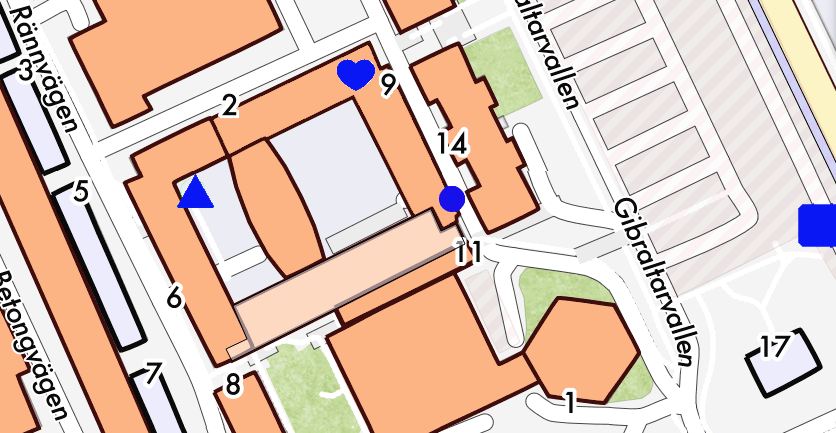
\includegraphics[scale=0.5, angle=90]{bokningsvillkor/map}
    \label{fig:map}
\end{figure}